% TMLR submission / arXiv preprint.
%
%   ANONYMOUS (for TMLR submission via OpenReview):  \usepackage{tmlr}
%   NAMED      (for the arXiv preprint):             \usepackage[preprint]{tmlr}
%   CAMERA-READY (after acceptance):                 \usepackage[accepted]{tmlr}
%
% Build both:  ./build.sh
\documentclass{article}

\usepackage{tmlr}
%\usepackage[preprint]{tmlr}
%\usepackage[accepted]{tmlr}

\usepackage{graphicx}
\usepackage{amsmath}
\usepackage{booktabs}
\usepackage{microtype}
\usepackage{url}
\usepackage[hidelinks]{hyperref}

% Expose the style file's preprint flag so identity-revealing text (code URL,
% acknowledgements) appears only in the non-anonymous builds.
\makeatletter
\newif\ifnamedbuild
\if@preprint\namedbuildtrue\fi
\if@accepted\namedbuildtrue\fi
\makeatother

\title{Tuberculosis Is Not in the Corner of the Image: Cross-Dataset Shortcut
Learning and the Limits of Lung Segmentation in Chest-Radiograph Classifiers}

\author{\name Alvin Chow \email alvinchow97@gmail.com \\
        \addr Independent Researcher}

\def\month{08}
\def\year{2026}
\def\openreview{\url{https://openreview.net/forum?id=XXXXXXXXXX}}

\begin{document}

\maketitle

\begin{abstract}
Deep networks achieve near-perfect tuberculosis (TB) detection on chest radiographs within a single
dataset, but such figures are rarely validated across institutions. We train a MobileNetV2
classifier on a widely used public TB radiography database and evaluate it, under a leakage-safe
protocol with bootstrap confidence intervals, on two independent National Library of Medicine
cohorts (Montgomery and Shenzhen). In-domain area under the ROC curve (AUC) reaches 0.9995 but
falls to 0.70--0.78 externally --- an approximately 0.25 AUC generalisation gap that five-fold
cross-validation confirms is stable ($0.25 \pm 0.02$). We decompose the accompanying collapse of
sensitivity to near zero into a threshold-transfer component (the optimal operating point shifts
roughly fivefold between sources) and a discrimination ceiling of about 70\% sensitivity at 70\%
specificity, and a duplicate-image audit establishes that the external cohorts share no overlap
with the training data. We then test the two most commonly recommended mitigations. Intensity
harmonisation with augmentation and multi-source training improves external AUC only marginally
($+0.02$). Lung segmentation, using a U-Net segmenter of high quality (Dice 0.975) producing
anatomically sound masks, fails to close the gap and degrades unbiased external AUC in every
cross-validation fold (paired decrease $0.057 \pm 0.011$), contrary to prior reports for COVID-19
radiography. The failure is moreover architecture-dependent: identically trained DenseNet-121 and
EfficientNet-B0 backbones match MobileNetV2 in-domain (all $\geq 0.999$) yet each collapses on a
\emph{different} external cohort (DenseNet to chance on Shenzhen, $0.503 \pm 0.025$; EfficientNet
to near-chance on Montgomery, $0.541 \pm 0.061$), so the two cohorts rank the three architectures
in entirely different orders. A frozen-feature probe shows these failure profiles already exist in
the ImageNet-pretrained representations before any fine-tuning, and masking homogenises all three
backbones into a common 0.61--0.77 band well below in-domain performance. We conclude that the
TB-CXR generalisation gap is real, large, and resistant to the standard playbook; that
single-cohort external validation can invert architecture rankings; and that out-of-source
validation on multiple cohorts is a prerequisite for trusting such models.
\end{abstract}

\section{Introduction}

Tuberculosis remains among the leading causes of death from infectious disease worldwide, and the
chest radiograph (CXR) is a primary screening modality, particularly where expert readers are
scarce. Convolutional networks have reported radiologist-level performance on CXR tasks
\citep{rajpurkar2017chexnet} and TB-specific AUCs as high as 0.99 \citep{lakhani2017deep},
motivating interest in automated TB screening.

Such headline figures, however, are usually obtained and reported on a single data source.
High in-distribution accuracy can reflect \emph{shortcut learning} \citep{geirhos2020shortcut}, in
which a model exploits dataset-specific cues that fail under distribution shift. In radiography
this is documented: a pneumonia classifier learned to detect a hospital-specific metal token
\citep{zech2018variable}, and COVID-19 classifiers were shown to rely on confounders rather than
pathology \citep{degrave2021ai}. Cross-dataset performance drops have also been reported for TB
classifiers trained on single-source archives
\citep{sathitratanacheewin2020deep, karki2022generalization, shuaibu2026geographic}. However, for
the multi-source composite database that has become the most widely used TB-CXR training benchmark
--- whose Normal and TB images are drawn from different source archives, an almost ideal setting
for shortcut learning --- the magnitude of the gap, its decomposition, and above all whether the
standard mitigations close it, remain unexamined.

This paper makes the following contributions.
\begin{enumerate}
\item We quantify the in-domain versus external generalisation gap for a standard TB-CXR classifier
with bootstrap confidence intervals under a leakage-safe evaluation protocol, and confirm its
stability with five-fold cross-validation and a duplicate-image audit.
\item We decompose the external failure into a threshold-transfer component and a discrimination
component.
\item We evaluate the two most-recommended mitigations --- intensity harmonisation with
augmentation and multi-source training, and lung segmentation --- and find that neither closes the
gap; segmentation, despite a high-quality segmenter, \emph{degrades} unbiased external performance
in every cross-validation fold, contradicting prior COVID-CXR findings \citep{bassi2022covid}.
\item We show the failure is architecture-dependent: DenseNet-121 and EfficientNet-B0 with
identical training match in-domain performance but each collapses on a \emph{different} external
cohort, inverting the architecture ranking between cohorts. A frozen-feature probe localises each
profile to the pretrained representation rather than to fine-tuning, and masking homogenises all
three backbones into a common sub-clinical band.
\item We draw the practical conclusion that out-of-source external validation on more than one
cohort is a prerequisite for trusting a TB-CXR model, and that neither segmentation nor any single
backbone should be assumed to confer robustness.
\end{enumerate}

\begin{figure}[t]
\centering
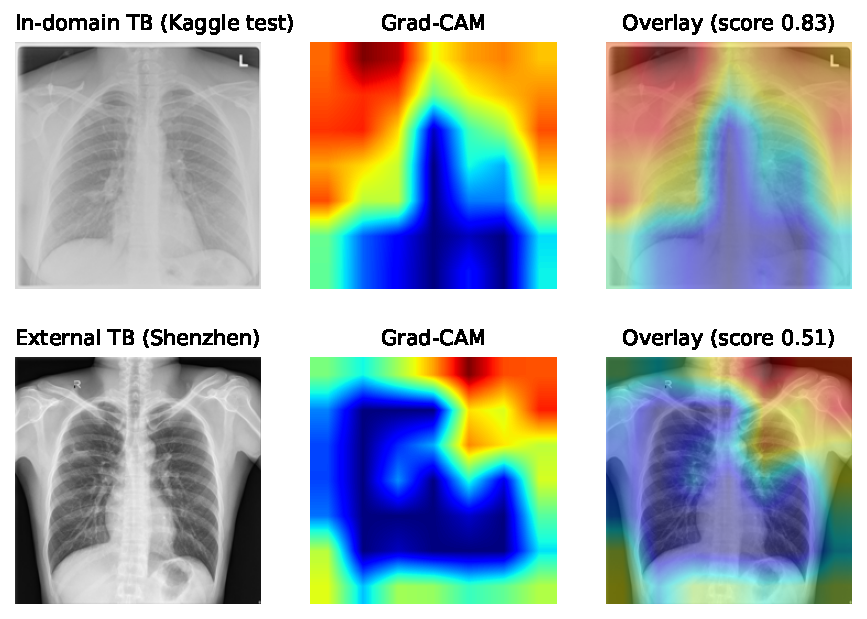
\includegraphics[width=0.92\textwidth]{figures/fig1_gradcam.pdf}
\caption{Grad-CAM attention for the baseline model. Top row: an in-domain TB case (score 0.83,
detected). Bottom row: a median-scoring external TB case (Shenzhen; score 0.51, below the 0.648
operating threshold and therefore missed). In both, attention falls largely on image borders and
the mediastinum rather than inside the lung fields --- qualitative evidence of shortcut reliance.}
\label{fig:gradcam}
\end{figure}

\section{Related Work}

\paragraph{Deep learning for chest radiography.}
\citet{rajpurkar2017chexnet} trained a 121-layer DenseNet on over 100{,}000 images and reported
pneumonia detection exceeding radiologist performance on a held-out set. For tuberculosis,
\citet{lakhani2017deep} obtained an AUC of 0.99 with ImageNet-pretrained CNNs. The systematic
review of \citet{hansun2023machine}, covering 47 studies, documents rapid growth alongside
recurring methodological weaknesses, notably limited external validation.

\paragraph{Shortcut learning and generalisation.}
\citet{geirhos2020shortcut} frame shortcut learning as decision rules that succeed on benchmarks
but fail out-of-distribution, with out-of-distribution testing as the diagnostic.
\citet{zech2018variable} found significant cross-hospital degradation for pneumonia and identified
a non-pathological confounder; \citet{degrave2021ai} showed COVID-19 classifiers relied on
confounders and argued explainability is a deployment prerequisite.

\paragraph{Cross-dataset TB validation.}
\citet{sathitratanacheewin2020deep} trained on the Shenzhen set and observed AUC fall from 0.85
(intramural) to 0.71 on NIH ChestX-ray8. \citet{karki2022generalization} reported a comparable drop
for drug-resistant TB and found that multi-task training with lesion-location supervision partially
recovered external performance. A recent multi-national study \citep{shuaibu2026geographic}
describes geographically divergent failure modes for a Shenzhen-trained DenseNet-121
(false-positive surge in a low-burden cohort, sensitivity collapse in a high-burden one). All of
these train on a single source archive and evaluate one architecture; none quantifies the gap for
the multi-source composite benchmark, tests lung segmentation as a mitigation, or examines whether
the failure is architecture-dependent --- the three axes of the present study.

\paragraph{Mitigations.}
Lung segmentation is the most advocated remedy, removing out-of-lung pixels:
\citet{bassi2022covid} reported it improved external COVID-19 performance and
\citet{teixeira2021impact} likewise found it important for COVID-19 generalisation, typically via a
U-Net \citep{ronneberger2015unet}. To our knowledge its effect on \emph{cross-dataset TB}
generalisation has not been tested. Harmonisation (e.g.\ contrast-limited adaptive histogram
equalisation) and augmentation target intensity cues. We evaluate both directly.

\paragraph{Evaluation rigour.}
\citet{rouzrokh2022mitigating} identify image-level (versus patient-level) splitting as a primary
source of optimistic bias, and \citet{tampu2022inflation} quantify inflation up to ${\sim}0.43$ in
Matthews correlation coefficient. These inform our interpretation of high in-domain figures and our
stated limitations.

\section{Materials and Methods}

\paragraph{Datasets.}
The in-domain data is the public TB Chest Radiography Database (3{,}500 Normal, 700 TB), split
80/10/10 with stratification. External validation uses two NLM cohorts \citep{jaeger2014two}:
Montgomery County (80 Normal, 58 TB) and Shenzhen Hospital (326 Normal, 336 TB). Montgomery
distributes ground-truth lung masks, used to train the segmenter. Source heterogeneity between
archives is the suspected origin of the confound.

\paragraph{Model and training.}
A MobileNetV2 backbone \citep{sandler2018mobilenetv2} pretrained on ImageNet is used with global
average pooling, dropout, and a sigmoid output. Images are preprocessed with the MobileNetV2
transform to $[-1, 1]$. Training is two-stage transfer learning (frozen-backbone head training,
then fine-tuning) with focal loss \citep{lin2017focal} to address the 5:1 class imbalance; gradient
clipping (clipnorm $= 1.0$) is applied for training stability.

\paragraph{Evaluation protocol.}
To avoid leakage, the operating threshold is selected on the validation set at sensitivity
$\geq 0.90$ and applied once to each test set. We report ROC-AUC and PR-AUC with 2{,}000-resample
bootstrap 95\% confidence intervals, plus sensitivity and specificity. Calibration is measured by
expected calibration error (ECE) with temperature scaling \citep{guo2017calibration} fitted on the
validation set. Grad-CAM \citep{selvaraju2017gradcam} and Integrated Gradients
\citep{sundararajan2017axiomatic} provide attention visualisations. Robustness is assessed by
five-fold stratified cross-validation, and data integrity by a duplicate-image audit (exact MD5
plus a 256-bit difference hash).

\paragraph{Mitigation A.}
CLAHE intensity harmonisation, stronger augmentation (rotation, zoom, translation, contrast),
reduced fine-tuning depth with increased dropout, and multi-source training under a
leave-one-dataset-out design (train on the composite database plus Shenzhen, hold out Montgomery).

\paragraph{Mitigation B.}
A U-Net \citep{ronneberger2015unet} lung segmenter is trained on the 138 Montgomery mask pairs with
a combined BCE--Dice loss. The trained segmenter masks all cohorts; a classifier identical to the
baseline except for masked input is trained on masked data. Shenzhen, unseen by the segmenter, is
the unbiased external test.

\paragraph{Backbone study and frozen-feature probe.}
To test whether the findings are specific to MobileNetV2, the five-fold cross-validation is
repeated with DenseNet-121 and EfficientNet-B0 backbones under an identical protocol --- the same
fold assignments, head architecture, two-stage training schedule, and focal loss --- with each
backbone paired with its own canonical input preprocessing, in both raw and masked-input
conditions. To localise the origin of any backbone-dependent behaviour, we additionally run a
frozen-feature probe: ImageNet-pretrained features are extracted from each backbone's
global-average-pooled output \emph{without any fine-tuning}, and an $L_2$-regularised logistic
regression is fitted on the training-split features and evaluated on the in-domain test split and
both external cohorts. Because the probe involves no gradient updates to the backbone, any external
failure it reproduces must be a property of the pretrained representation interacting with the
dataset shift, not of the training procedure. As a low-level check, we also measure the
discriminative power of mean image brightness alone per cohort, and the Spearman correlation
between each probe's scores and image brightness.

\section{Results}

\subsection{Generalisation gap}
In-domain test AUC was 0.9995 (95\% CI 0.998--1.000; PR-AUC 0.998), falling to 0.776 (0.740--0.811)
on Shenzhen, 0.698 (0.607--0.784) on Montgomery, and 0.752 (0.719--0.786) pooled
(Table~\ref{tab:gap}). Confidence intervals for the external cohorts do not overlap the in-domain
estimate; an unpaired bootstrap difference confirms the in-domain--Shenzhen gap is significant
($\Delta = 0.22$, 95\% CI 0.19--0.26, $p < 0.001$). The corresponding ROC curves are shown in
Figure~\ref{fig:roc}.

\begin{table}[t]
\caption{In-domain versus external discrimination (95\% bootstrap confidence intervals).}
\label{tab:gap}
\centering
\begin{tabular}{lccc}
\toprule
Evaluation & ROC-AUC (95\% CI) & Sens. & Spec. \\
\midrule
In-domain (composite DB) & 0.9995 (0.998--1.000) & 0.93 & 1.00 \\
Shenzhen & 0.776 (0.740--0.811) & 0.02 & 1.00 \\
Montgomery & 0.698 (0.607--0.784) & 0.00 & 1.00 \\
Combined & 0.752 (0.719--0.786) & 0.02 & 1.00 \\
\bottomrule
\end{tabular}
\end{table}

\begin{figure}[t]
\centering
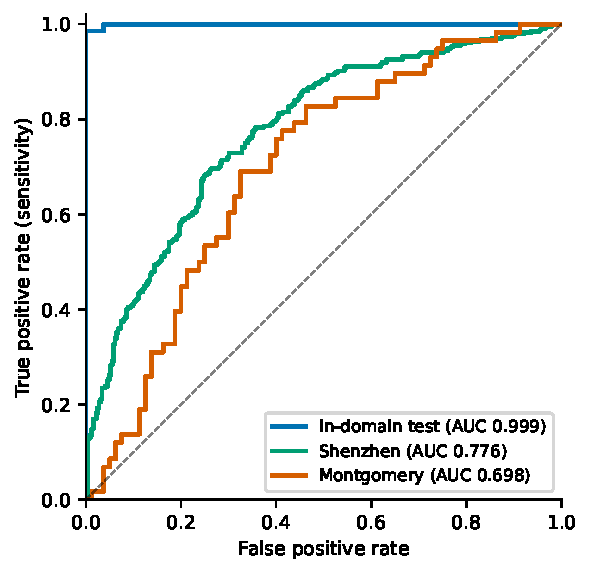
\includegraphics[width=0.55\textwidth]{figures/fig2_roc.pdf}
\caption{ROC curves for the baseline classifier: in-domain test (AUC 0.9995) versus Montgomery
(0.698) and Shenzhen (0.776), illustrating the ${\sim}0.25$ AUC generalisation gap.}
\label{fig:roc}
\end{figure}

\subsection{Threshold versus discrimination}
At the in-domain threshold (0.648) external sensitivity was ${\approx}0$; the model required
thresholds of 0.05--0.23 externally. At a balanced (Youden) operating point the cohorts reached
${\approx}0.71/0.69$ (combined) sensitivity/specificity (Table~\ref{tab:threshold}), indicating the
collapse is partly threshold-transfer and partly a discrimination ceiling.

\begin{table}[t]
\caption{External performance by operating point.}
\label{tab:threshold}
\centering
\begin{tabular}{lccc}
\toprule
Cohort & AUC & thr 0.648 (se/sp) & Youden (se/sp) \\
\midrule
Montgomery & 0.698 & 0.00 / 1.00 & 0.83 / 0.54 \\
Shenzhen & 0.776 & 0.02 / 1.00 & 0.68 / 0.75 \\
Combined & 0.752 & 0.02 / 1.00 & 0.71 / 0.69 \\
\bottomrule
\end{tabular}
\end{table}

\subsection{Calibration}
ECE was 0.770 before and 0.833 after temperature scaling (fitted $T = 0.12$); the perfectly
separated validation set makes the fit degenerate, so calibration could not be corrected
(Figure~\ref{fig:reliability}).

\begin{figure}[t]
\centering
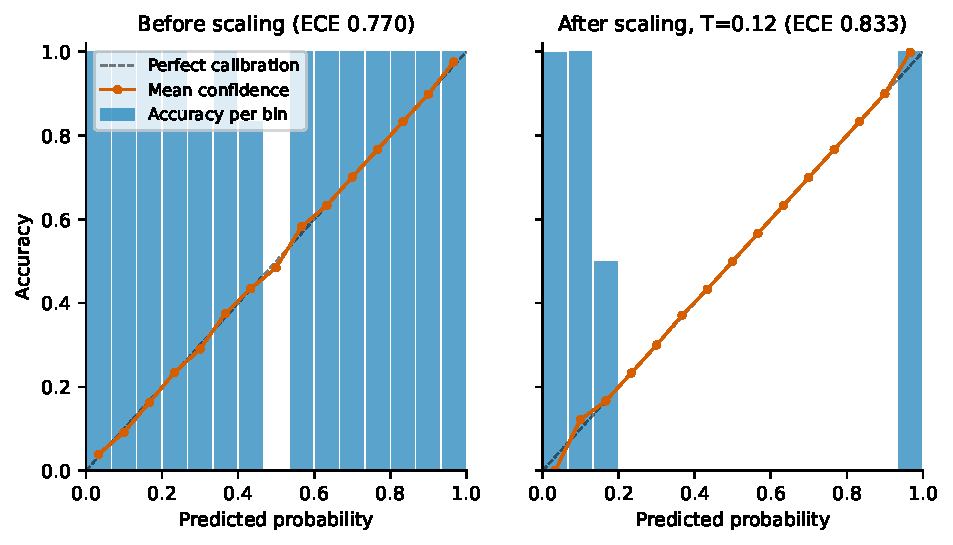
\includegraphics[width=0.92\textwidth]{figures/fig3_reliability.pdf}
\caption{Reliability diagrams on the in-domain test set, before (ECE 0.770) and after (ECE 0.833)
temperature scaling, showing that scaling fails to correct the over-confident, saturated
probabilities.}
\label{fig:reliability}
\end{figure}

\subsection{Mitigation A: harmonisation, augmentation, multi-source training}
External (Montgomery) AUC improved from 0.698 to 0.719 ($+0.021$) while in-domain fell from 0.999
to 0.966 (Table~\ref{tab:mitigations}); the gap narrowed chiefly through reduced over-fitting.

\subsection{Mitigation B: lung segmentation}
The segmenter achieved validation Dice 0.975; retained lung-pixel fractions were 0.26--0.31 across
all cohorts (Shenzhen 0.29) with no degenerate masks (Figure~\ref{fig:segmentation}). On the
primary split, masked-input AUC was 0.998 in-domain, 0.728 on Montgomery (confounded; segmenter
trained on Montgomery), and 0.662 on Shenzhen --- a decrease of 0.114 versus the raw baseline on
the unbiased cohort (Table~\ref{tab:mitigations}), significant by DeLong's test for correlated ROC
curves ($z = 4.65$, $p < 0.001$). The cross-validated, fold-paired comparison confirms the direction
while tempering the magnitude: masking reduced Shenzhen AUC in \textbf{all five folds} (raw
$0.743 \pm 0.030$ versus masked $0.686 \pm 0.030$; paired decrease $0.057 \pm 0.011$, paired
$t = 11.9$, $p < 0.001$), whereas the Montgomery difference was not consistent across folds (mean
$-0.009$, mixed signs). We therefore report the cross-validated paired decrease of ${\approx}0.06$
AUC as the primary estimate of the segmentation penalty, with the single-split value of 0.114 as
one realisation. Section~\ref{sec:backbones} shows this penalty is specific to the MobileNetV2
backbone: for architectures whose raw external transfer had collapsed, the same masking instead
\emph{recovers} performance --- into the same mediocre band.

\begin{table}[t]
\caption{Mitigation results (AUC). Shenzhen is the unbiased external cohort, unseen by the
segmenter.}
\label{tab:mitigations}
\centering
\begin{tabular}{lccc}
\toprule
Condition & In-domain & Montgomery & Shenzhen \\
\midrule
Baseline (raw) & 0.999 & 0.698 & 0.776 \\
Mitigation A & 0.966 & 0.719 & --- \\
Mitigation B (masked) & 0.998 & 0.728 & 0.662 \\
\bottomrule
\end{tabular}
\end{table}

\begin{figure}[t]
\centering
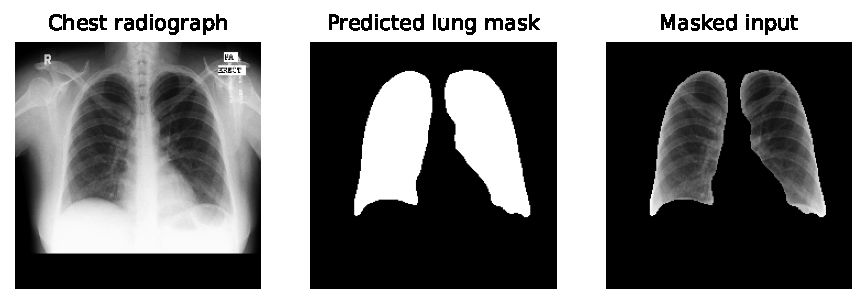
\includegraphics[width=0.92\textwidth]{figures/fig4_segmentation.pdf}
\caption{Lung segmentation example: original chest radiograph, U-Net predicted lung mask, and the
resulting masked input fed to the classifier (Dice 0.975 on held-out Montgomery masks).}
\label{fig:segmentation}
\end{figure}

\subsection{Robustness: five-fold cross-validation}
To confirm the gap is not an artefact of a single split, we ran five-fold stratified
cross-validation on the in-domain data, evaluating each fold's model on the fixed external cohorts
(Table~\ref{tab:cv}). The gap is stable: in-domain AUC $0.9991 \pm 0.0009$, Montgomery
$0.6884 \pm 0.0040$, Shenzhen $0.7461 \pm 0.0215$, giving a generalisation gap (in-domain minus
Shenzhen) of $0.2530 \pm 0.0223$. The small per-fold variance --- Montgomery ranged only
0.682--0.694 --- indicates the gap is a stable property of the source mismatch rather than of any
particular split.

\begin{table}[t]
\caption{Five-fold cross-validation (AUC, mean $\pm$ std).}
\label{tab:cv}
\centering
\begin{tabular}{lc}
\toprule
Evaluation & AUC (mean $\pm$ std) \\
\midrule
In-domain & $0.9991 \pm 0.0009$ \\
Montgomery & $0.6884 \pm 0.0040$ \\
Shenzhen & $0.7461 \pm 0.0215$ \\
Gap (in-domain $-$ Shenzhen) & $0.2530 \pm 0.0223$ \\
\bottomrule
\end{tabular}
\end{table}

\subsection{Data-overlap audit}
Because the in-domain AUC is near-perfect, we audited for duplicate leakage using exact MD5 hashing
and a discriminative 256-bit difference hash (a coarse hash over-reports duplicates for
radiographs, which share gross structure). Within the composite database, only two byte-identical
files and a small number of near-duplicate pairs (Hamming $\leq 10$, all within-class) span the
train/test boundary, affecting ${\approx}1\%$ of the test set --- far too few to account for the
in-domain AUC, which instead reflects genuine within-source separability. The cross-cohort check
deserves particular care because the composite database's own documentation lists the NLM
Montgomery and Shenzhen collections among its candidate sources \citep{rahman2020reliable}: if the
public release actually contained those images, our ``external'' cohorts would not be external at
all. Three independent checks refute this for the public release used here. No exact (MD5) or
near-duplicate (Hamming $\leq 10$) hash overlap was found between the composite database and either
external cohort (nearest distances 29 and 40 for Montgomery and Shenzhen). A complementary
normalised cross-correlation scan of every external image against the entire release
($64 \times 64$ grayscale) found no pair above 0.93, and visual inspection of the top-ranked pairs
confirmed they are different patients --- the observed maxima reflect the generic similarity of
chest radiographs, not reprocessed duplicates. We conclude the public release draws its TB images
from the non-NLM portals and that the generalisation gap is a true out-of-source failure, not an
artefact of data contamination.

\subsection{Backbone dependence and the frozen-feature probe}
\label{sec:backbones}
Repeating the five-fold protocol with DenseNet-121 and EfficientNet-B0 backbones leaves in-domain
discrimination unchanged (all three $\geq 0.999$) but produces three qualitatively different
external profiles (Table~\ref{tab:backbones}). DenseNet-121 falls to chance on Shenzhen
($0.503 \pm 0.025$) while \emph{improving} over MobileNetV2 on Montgomery ($0.746 \pm 0.020$ versus
$0.693 \pm 0.011$); EfficientNet-B0 shows the mirror-image failure, falling to near chance on
Montgomery ($0.541 \pm 0.061$) while retaining moderate discrimination on Shenzhen
($0.659 \pm 0.015$). The two external cohorts therefore rank the three architectures in entirely
different orders (Montgomery: DenseNet $>$ MobileNet $>$ EfficientNet; Shenzhen:
MobileNet $>$ EfficientNet $>$ DenseNet), with each backbone collapsing on a different cohort.

The frozen-feature probe shows this divergence is not created by fine-tuning: a logistic regression
on frozen ImageNet features alone reproduces each backbone's profile (MobileNetV2: 0.9996
in-domain / 0.738 Montgomery / 0.768 Shenzhen; DenseNet-121: 0.9965 / 0.780 / 0.571;
EfficientNet-B0: 0.9995 / 0.598 / 0.684), so each architecture's external failure pre-exists in its
pretrained representation, and fine-tuning merely amplifies it (e.g.\ DenseNet--Shenzhen
$0.571 \rightarrow 0.503$; EfficientNet--Montgomery $0.598 \rightarrow 0.541$). A low-level
analysis suggests a partial mechanism: mean image brightness alone is uninformative in-domain
(AUC 0.52) but anti-correlated with TB on Shenzhen (AUC 0.34; TB films are systematically darker),
and the DenseNet probe's scores correlate \emph{positively} with brightness on Shenzhen (Spearman
$\rho = +0.15$, $p < 10^{-4}$) --- the wrong direction --- whereas MobileNetV2's correlate
negatively ($\rho = -0.12$, $p = 0.003$). The correlations are weak, so brightness is a
contributing cue rather than a complete explanation; the substantive point is that different
pretrained representations expose different shortcut directions, with opposite consequences on
different external cohorts.

The masked-input condition (Table~\ref{tab:backbones}, lower half) reveals that the segmentation
effect is itself backbone-dependent --- and in a structured way. Masking significantly
\emph{degrades} the best raw transfer (MobileNetV2--Shenzhen: $-0.057 \pm 0.011$, paired
$t = -11.9$, $p < 0.001$) yet significantly \emph{recovers} the collapsed ones
(DenseNet-121--Shenzhen: $+0.109 \pm 0.044$, $p = 0.005$; EfficientNet-B0--Montgomery:
$+0.226 \pm 0.075$, $p = 0.003$). The net effect is homogenisation: masking compresses the
between-backbone spread of external AUC from 0.21--0.24 to 0.07--0.08, pulling all three
architectures into a common 0.61--0.77 band regardless of where they started --- well below
in-domain performance. This is consistent with masking removing the backbone-specific shortcut cues
(both the helpful and the catastrophic ones) while capping performance at whatever
lung-field-only signal transfers across sources.

\begin{table}[t]
\caption{Backbone study: five-fold cross-validation (AUC, mean $\pm$ std), raw and masked input.
The MobileNetV2 raw row re-estimates the Table~\ref{tab:cv} cross-validation under the
backbone-study pipeline (batch size 16 rather than 32); the two agree within fold variance.}
\label{tab:backbones}
\centering
\begin{tabular}{llccc}
\toprule
Backbone & Input & In-domain & Montgomery & Shenzhen \\
\midrule
MobileNetV2 & raw & $0.9991 \pm 0.0012$ & $0.6926 \pm 0.0109$ & $0.7426 \pm 0.0295$ \\
DenseNet-121 & raw & $0.9994 \pm 0.0004$ & $0.7458 \pm 0.0203$ & $0.5032 \pm 0.0248$ \\
EfficientNet-B0 & raw & $0.9993 \pm 0.0011$ & $0.5406 \pm 0.0614$ & $0.6585 \pm 0.0148$ \\
\midrule
MobileNetV2 & masked & $0.9915 \pm 0.0062$ & $0.7016 \pm 0.0327$ & $0.6859 \pm 0.0296$ \\
DenseNet-121 & masked & $0.9907 \pm 0.0078$ & $0.7448 \pm 0.0198$ & $0.6118 \pm 0.0280$ \\
EfficientNet-B0 & masked & $0.9968 \pm 0.0031$ & $0.7669 \pm 0.0184$ & $0.6882 \pm 0.0144$ \\
\bottomrule
\end{tabular}
\end{table}

\begin{figure}[t]
\centering

\includegraphics[width=0.98\textwidth]{figures/fig5_backbones.pdf}
\caption{External generalisation is backbone-dependent. Grouped bars: AUC per cohort (in-domain
test, Montgomery, Shenzhen) for each backbone, fine-tuned (solid, five-fold mean $\pm$ std) and
frozen-feature probe (hatched). All three backbones are indistinguishable in-domain, yet each
collapses on a different external cohort (DenseNet-121 on Shenzhen, EfficientNet-B0 on
Montgomery), and every frozen probe reproduces its backbone's fine-tuned profile --- the failures
are inherited from pretraining, not induced by fine-tuning.}
\label{fig:backbones}
\end{figure}

\section{Discussion}

The gap's magnitude and the fivefold threshold shift match the shortcut-learning signature
described for pneumonia \citep{zech2018variable} and COVID-19 \citep{degrave2021ai}; against the
external benchmarks of \citet{han2025systematic} (${\approx}0.85$--$0.97$ for deployable systems)
the unmitigated model (${\approx}0.75$) is below clinical usefulness.
Table~\ref{tab:priorwork} situates our result among representative prior TB-CXR studies and
highlights that the strongest reported figures are predominantly in-domain, with independent
cross-source external validation reported far less often --- the very gap this study foregrounds.

\begin{table}[t]
\caption{Reported TB-CXR performance and external-validation status (as-reported; datasets differ,
so figures are not directly comparable).}
\label{tab:priorwork}
\centering
\small
\begin{tabular}{p{3.1cm}p{3.5cm}p{3.4cm}p{3.0cm}}
\toprule
Study & Approach & Reported AUC & Cross-source external test? \\
\midrule
\citet{lakhani2017deep} & AlexNet/GoogLeNet & 0.99 (in-domain) & Not reported as held-out
external \\
\citet{rahman2020reliable} & CNNs $+$ segmentation (same DB) & ${\sim}0.99$ & No (same source) \\
\citet{sathitratanacheewin2020deep} & DCNN (Shenzhen-trained) & 0.85 in-domain / 0.71 external &
Yes (one cohort) \\
\citet{karki2022generalization} & CNNs, multi-task (DR-TB) & ${\sim}0.85$ in-domain / 0.65
external & Yes \\
\citet{han2025systematic} (meta) & Various & 0.85--0.97 (external) & Yes \\
\textbf{This work} & MobileNetV2, DenseNet-121, EfficientNet-B0 & 0.999 in-domain / 0.50--0.78
external & \textbf{Yes (two cohorts)} \\
\bottomrule
\end{tabular}
\end{table}

Mitigation A regularised the model without supplying cross-domain invariance, narrowing the gap
mainly by reducing in-domain over-fitting. The segmentation result is the most striking: because
masks were verified (Dice 0.975; plausible lung fractions on every cohort), failed segmentation is
excluded. The backbone study sharpens the interpretation: masking degrades the backbone whose raw
transfer was best yet recovers those that had collapsed, compressing all three into a common
0.61--0.77 band. This is what one would expect if masking removes \emph{backbone-specific} cues
outside the lung fields --- both the accidentally helpful and the catastrophically misleading ones
--- while the lung-field-only signal that survives transfers only partially across sources. What
masking cannot do, on any backbone, is approach in-domain performance, so it is not a remedy for
the gap; whether the residual ceiling reflects genuinely limited transferable pathology signal or
residual within-lung confounds remains for future testing. The divergence from
\citet{bassi2022covid} may reflect task and cohort differences, cautioning against assuming a
mitigation validated on one disease transfers to another. Clinically, the failure mode is missed
disease (false negatives), the costlier error in screening, and the threshold is non-transferable,
so target-domain recalibration would be required.

The backbone study adds a second cautionary layer. In-domain performance is indistinguishable
across architectures (all $\geq 0.999$), yet external behaviour diverges to the point that each
backbone collapses on a \emph{different} cohort and the two cohorts rank the three architectures in
entirely different orders. Had this study used only one external cohort --- the common practice
when external validation is performed at all --- the conclusion about which architecture
generalises better would have depended entirely on which cohort was chosen. The frozen-feature
probe traces the divergence to the pretrained representations themselves: each ImageNet encoder
projects the radiographs into a feature space whose in-domain-separable directions align
differently with each external cohort's covariate shift, in line with the view of shortcut learning
as an interaction between inductive bias and data \citep{geirhos2020shortcut}. Practically, the
probe is inexpensive --- it requires no fine-tuning --- and could serve as a pre-deployment
diagnostic: if frozen features already rank an external cohort poorly, no amount of head training
on the source domain should be expected to fix it. The partial brightness mechanism also suggests
trivial photometric normalisation checks belong in any TB-CXR evaluation protocol.

\paragraph{Limitations.}
The composite database lacks patient identifiers, so although our duplicate-image audit found
negligible image-level overlap, residual same-patient leakage across the train/test boundary cannot
be fully excluded; the near-perfect in-domain figures should be read with this caveat
\citep{rouzrokh2022mitigating, tampu2022inflation}. The segmenter was trained on Montgomery,
confounding that cohort, so Shenzhen is treated as the primary external test. Only two mitigation
families were evaluated, and all data are retrospective and public. The backbone study covers three
ImageNet-pretrained convolutional encoders; transformer-based and radiograph-pretrained encoders
remain untested, and the brightness correlation explains only part of the DenseNet--Shenzhen
failure, whose full mechanism is left open.

\section{Conclusion}

A standard TB-CXR classifier achieved near-perfect in-domain AUC yet lost ${\approx}0.25$ AUC on
independent cohorts --- a gap confirmed stable by five-fold cross-validation and not attributable
to data contamination --- and it resisted both standard mitigations, with harmonisation and
augmentation giving only a marginal gain and lung segmentation degrading unbiased external
performance in every cross-validation fold despite a high-quality segmenter. The failure is
moreover architecture-dependent: DenseNet-121 and EfficientNet-B0, indistinguishable in-domain,
each fell to chance or near-chance on a different external cohort, a divergence a frozen-feature
probe traces to the pretrained representations themselves; and masking homogenised all three
backbones into a common sub-clinical band, degrading the best transfer while recovering the
collapsed ones. We conclude that strong in-domain numbers are not evidence of generalisation, that
out-of-source external validation --- on more than one cohort --- is necessary before trusting a
TB-CXR model, and that neither lung segmentation nor backbone choice validated on a single cohort
is a guaranteed remedy. Future work should establish patient-level splits, train multi-domain
segmenters, evaluate domain-adversarial and test-time adaptation, and test whether
radiograph-pretrained encoders escape the shortcut directions that ImageNet encoders inherit.

\section*{Broader Impact Statement}

This work studies automated tuberculosis screening, a setting where deployment errors carry direct
human cost. Our findings are cautionary rather than capability-advancing: we show that a classifier
reporting near-perfect accuracy on its source dataset can miss essentially all disease on an
independent cohort at its nominal operating threshold. The intended positive impact is to
discourage premature deployment of TB-CXR models validated on a single data source, and to
establish that neither lung segmentation nor a change of backbone should be assumed to confer
robustness.

The most salient risk we identify is asymmetric: the observed failure mode is false negatives,
meaning missed disease in a screening population that is frequently under-served, so an
over-trusted model could delay treatment for exactly the patients such systems are promoted to
help. We report the threshold-transfer effect explicitly so that practitioners understand that an
operating point tuned on source data does not transfer, and that target-domain recalibration is
mandatory rather than optional.

A secondary risk attaches to the mitigation results. Because we report that segmentation can
\emph{recover} performance for backbones whose transfer had collapsed, these numbers should not be
read as endorsing masked-input models for deployment: every masked configuration we measured
remained far below in-domain performance and below published thresholds for clinically useful
systems. We recommend that no configuration reported here be used for patient care. All data used
are public, de-identified, retrospective research datasets; no new patient data were collected and
no human subjects were involved, so no IRB review was required.

\ifnamedbuild
\section*{Reproducibility Statement}

All experiments use public datasets and are reproducible from the released code. The repository
contains the training and evaluation notebook, the backbone-study script (which verifies its
reproduced data split against a cached reference before training and is resumable per fold), the
frozen-feature probe, the figure-generation script, pinned dependency versions, and the raw
per-fold result files underlying every table. Random seeds are fixed and reported; per-fold seeds
are derived deterministically. Code: \url{https://github.com/alvinchow97/tb-xray-analysis}.
\else
\section*{Reproducibility Statement}

All experiments use public datasets. Code accompanying this submission --- the training and
evaluation notebook, the backbone-study script (which verifies its reproduced data split against a
cached reference before training and is resumable per fold), the frozen-feature probe, the
figure-generation script, pinned dependency versions, and the raw per-fold result files underlying
every table --- is provided as anonymised supplementary material and will be released publicly upon
acceptance. Random seeds are fixed and reported; per-fold seeds are derived deterministically.
\fi

\bibliographystyle{tmlr}
\bibliography{references}

\end{document}
